\documentclass[24pt,pdf,hyperref={unicode},aspectratio=169]{beamer}
\usepackage[utf8]{inputenc}
\usepackage{aiml}
\usetikzlibrary{calc}
\usetikzlibrary{shapes.geometric}

\begin{document}
\section{Реализация нейронных сетей}
\begin{frame}\frametitle{Матричная запись персептрона}

\begin{tikzpicture}[shorten >=1pt,->,draw=black!50, node distance=\layersep]
     \tikzstyle{every pin edge}=[<-,shorten <=1pt]
     \tikzstyle{neuron}=[circle,fill=black!25,minimum size=17pt,inner sep=0pt]
     \tikzstyle{input neuron}=[neuron, fill=green!50];
     \tikzstyle{output neuron}=[neuron, fill=red!50];
     \tikzstyle{hidden neuron}=[neuron, fill=blue!50];
     \tikzstyle{annot} = [text width=4em, text centered]
 
 	
 	\foreach \num in {1,...,5}
 		\node (x-\num) at (0,5-\num) {$x_{\num}$};
 		
 	\foreach \num in {1,...,4}
 	{
 		\node[neu] (n-\num) at (2,4.5-\num) {};
 		\node (y-\num) at (3,4.5-\num) {$y_{\num}$};
 		\path (n-\num) edge (y-\num);
 	}
 	
 	\foreach \num in {1,...,5}
 	{
	 	\node[neu] (m-\num) at (5,5-\num) {};
 	 	\node (z-\num) at (6,5-\num) {$z_{\num}$};
 	 	\path (m-\num) edge (z-\num);
 	}
 	
 	
 	\foreach \num in {1,...,3}
 	{
	 	\node[neu] (p-\num) at (8,4-\num) {};
 	 	\node (o-\num) at (9,4-\num) {$o_{\num}$};
 	 	\path (p-\num) edge (o-\num);
 	} 	
 	
 	\foreach \st in {1,...,5} \foreach \ds in {1,...,4} \path (x-\st) edge (n-\ds);
 	\foreach \st in {1,...,4} \foreach \ds in {1,...,5} \path (y-\st) edge (m-\ds);
 	\foreach \st in {1,...,5} \foreach \ds in {1,...,3} \path (z-\st) edge (p-\ds);
\end{tikzpicture}

$$
O=F(W_1\times F(W_2\times F(W_3\times X)))
$$
\end{frame}


\begin{frame}\frametitle{Аналоговая нейронная сеть}
\begin{center}
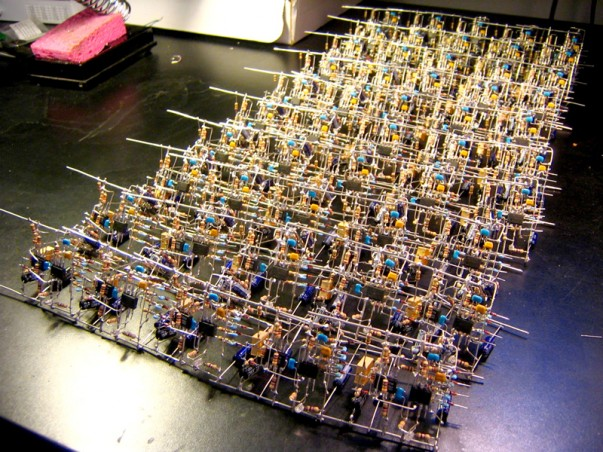
\includegraphics[width=0.7\textwidth]{Images/AnalogNN.jpg}
\end{center}
\end{frame}

\begin{frame}\frametitle{Аналоговая нейронная сеть}
\begin{center}
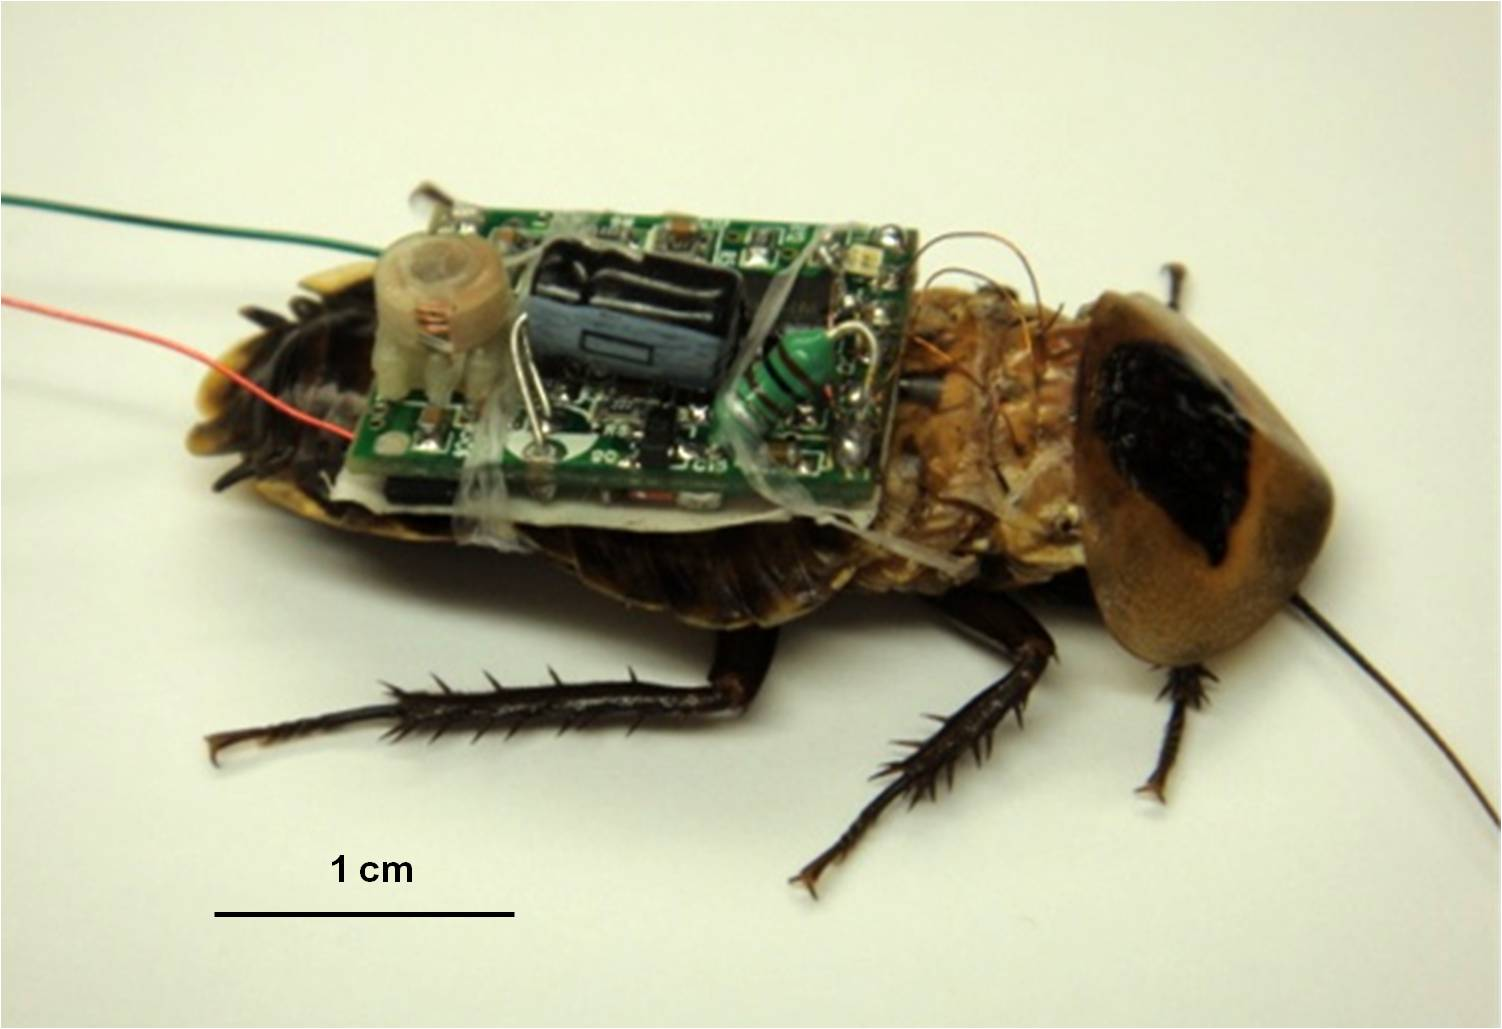
\includegraphics[width=0.7\textwidth]{Images/cyborg.jpg}
\end{center}
\end{frame}


\end{document}
\end{document}